% begin module tangents-alternative-form
\begin{frame}
\begin{columns}[c]
\column{.4\textwidth}
\ \only<handout:0| -1,12->{%
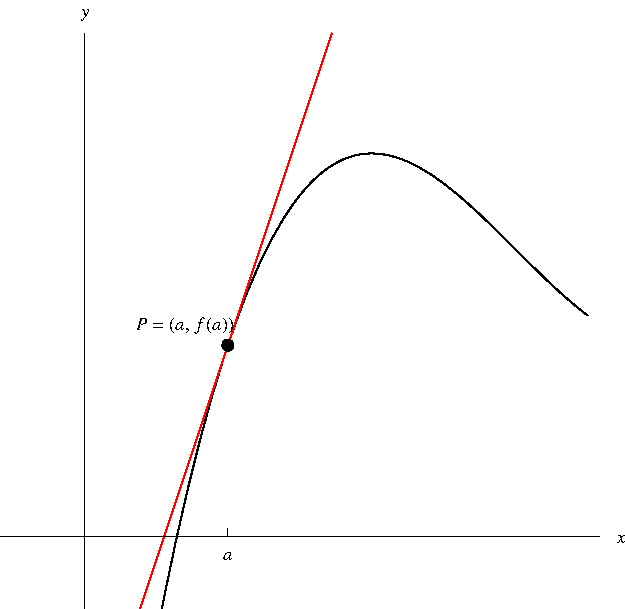
\includegraphics[height=4.5cm]{derivatives/pictures/03-01-tangent.pdf}%
}%
\only<handout:1| 2>{%
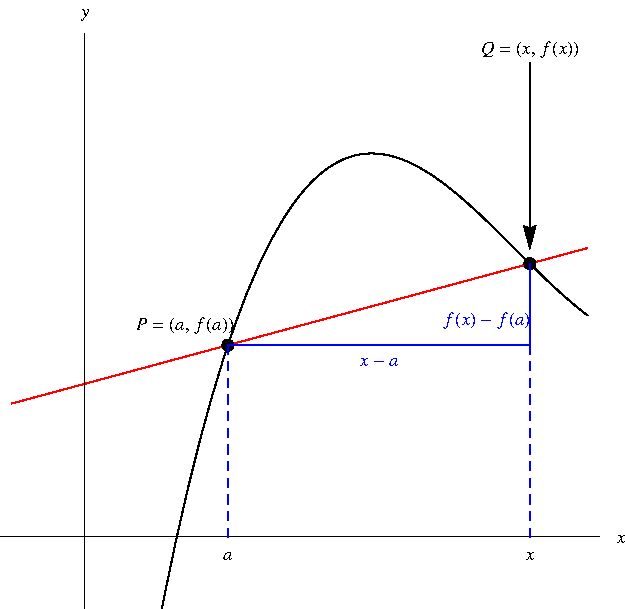
\includegraphics[height=4.5cm]{derivatives/pictures/03-01-secanta.pdf}%
}%
\only<handout:2-| 3-5>{%
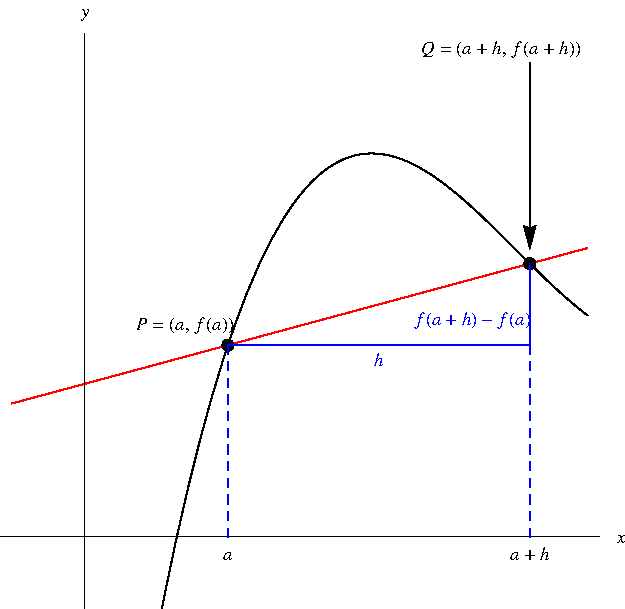
\includegraphics[height=4.5cm]{derivatives/pictures/03-01-secantha.pdf}%
}%
\only<handout:0| 6>{%
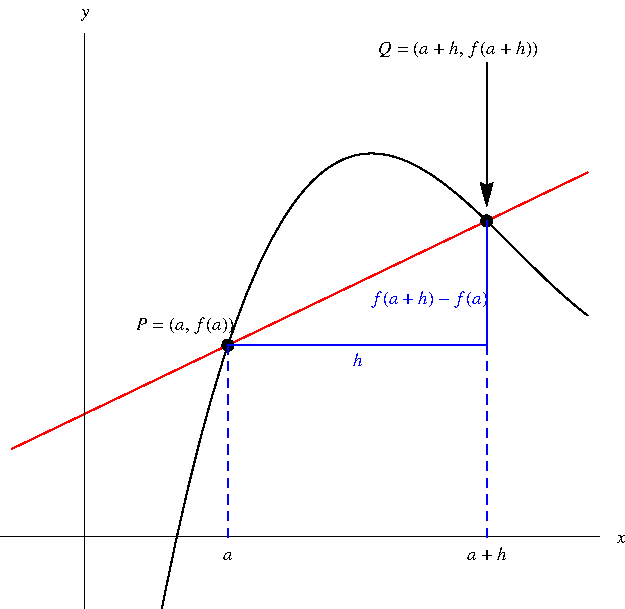
\includegraphics[height=4.5cm]{derivatives/pictures/03-01-secanthb.pdf}%
}%
\only<handout:0| 7>{%
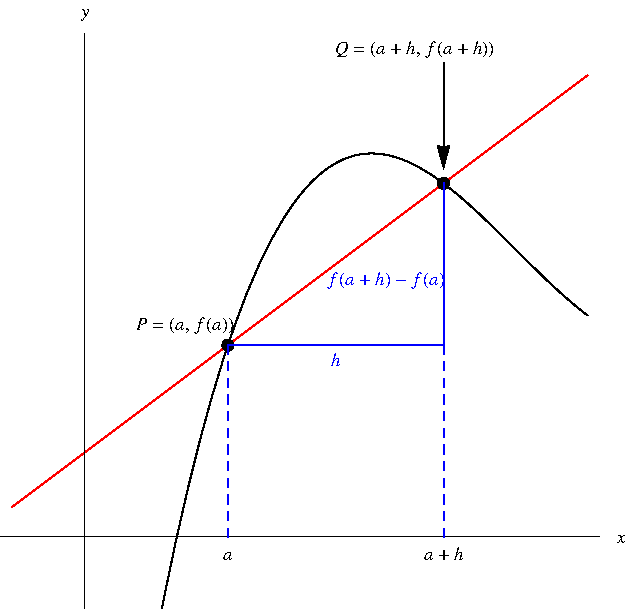
\includegraphics[height=4.5cm]{derivatives/pictures/03-01-secanthc.pdf}%
}%
\only<handout:0| 8>{%
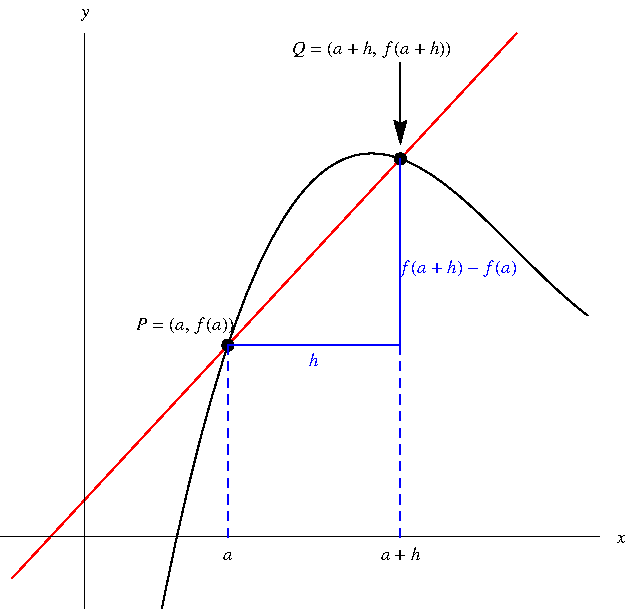
\includegraphics[height=4.5cm]{derivatives/pictures/03-01-secanthd.pdf}%
}%
\only<handout:0| 9>{%
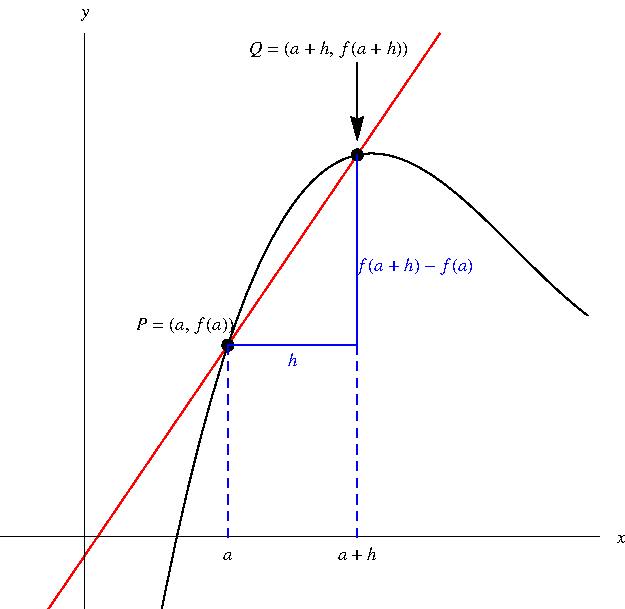
\includegraphics[height=4.5cm]{derivatives/pictures/03-01-secanthe.pdf}%
}%
\only<handout:0| 10>{%
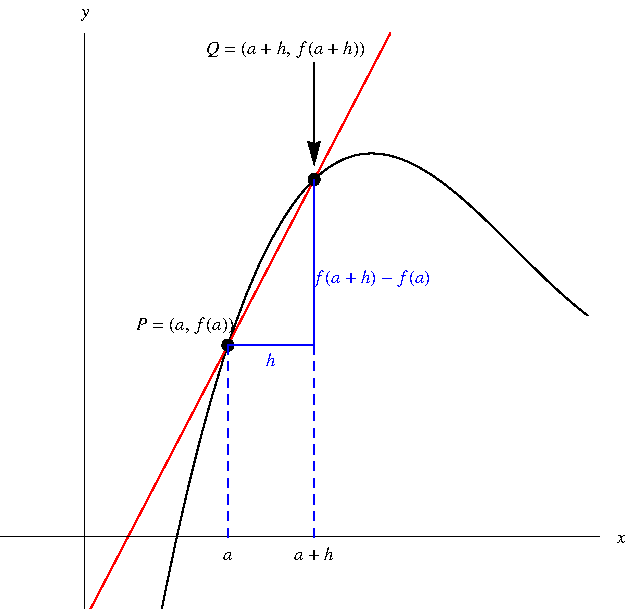
\includegraphics[height=4.5cm]{derivatives/pictures/03-01-secanthf.pdf}%
}%
\only<handout:0| 11>{%
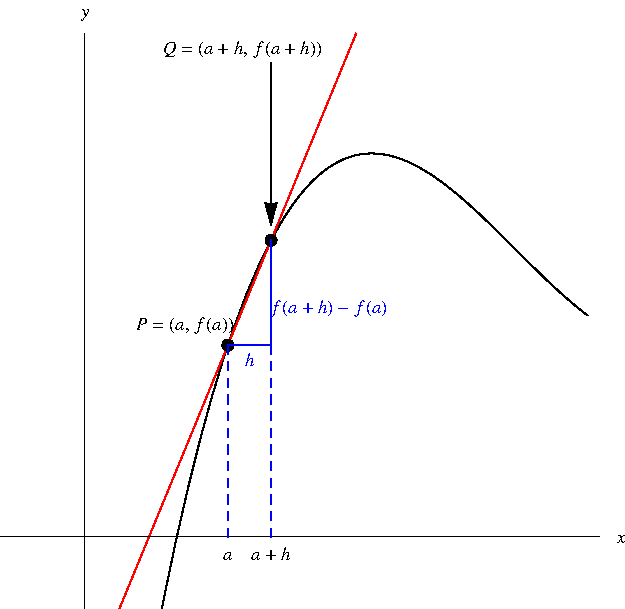
\includegraphics[height=4.5cm]{derivatives/pictures/03-01-secanthg.pdf}%
}%
\column{.6\textwidth}
\begin{itemize}
\item<1->  There is another expression for the slope of the tangent line.
\item<2->  Our definition involves letting $x$ tend to $a$.
\item<handout:2-| 3->  Instead, think in terms of $h = x - a$.
\item<handout:2-| 4->  Then $x = a+h$ and the slope of the secant line $PQ$ is $m_{PQ} = \frac{f(a+h)-f(a)}{h}$.
\item<handout:2-| 5->  We still view the slope as a limit, only now in terms of the quantity $h$.
\end{itemize}
\end{columns}

\uncover<handout:2-| 12->{%
Alternative formula:
\[
m = \lim_{h\rightarrow 0}\frac{f(a+h) - f(a)}{h}.
\]
}%
\end{frame}
% end module tangents-alternative-form
